\chapter{Описание реализации метода частиц в ячейках для высокопроизводительных ВС}
\label{chapt1}

\section{Краткое описание метода частиц в ячейках}


Основываясь на
\cite{VshivkovPICbook}, приведем описание основной идеи метода. Пусть задача записана 
в абстрактной операторной форме:
\begin{equation}
\label{Abs1}
\frac{\partial \textbf{q}}{\partial t} + A\textbf{q} = 0.
\end{equation}

Решение задачи (\ref{Abs1}) представляется в виде следующей интерполяционной 
формулы:
\begin{equation}
\label{AbsInt}
\textbf{q} = \sum\limits^{N}_{j=1}\textbf{Q}_j R(\textbf{u},\textbf{u}_j(t)).
\end{equation}
Этот переход называют разбиением среды на модельные частицы. Функция 
$R(\textbf{u},\textbf{v})$ называется ядром модельной частицы. Представление
(\ref{AbsInt}) позволяет свести решение задачи 
(\ref{Abs1}) к интегрированию динамической системы частиц.


\quad Система уравнений движения модельных частиц получается
\cite{VshivkovPICbook} из уравнения Власова подстановкой функции
распределения в виде
\begin{equation}\label{fr}
f(t,x,u)=\sum_{j=1}^m R(x-x_j(t))\delta(u-u_j(t))
\end{equation}
где $R$ -- произвольное сеточное ядро,  %ядро модельной частицы,
$\delta$ -- дельта-функция, $m$ -- полное число модельных частиц.

Для удобства будем рассматривать наши уравнения в безразмерных
величинах
\begin{equation}\label{dx}
\frac{dx_j(t)}{dt}=u_j(t),
\end{equation}
\begin{equation}\label{du}
\frac{du_j(t)}{dt}=E(x_j),
\end{equation}
\begin{displaymath}
j=1,\ldots, m
\end{displaymath}
- уравнения движения частиц (совпадают с уравнениями характеристик
кинетического уравнения Власова).

\section{Модель высокотемпературной бесстолкновительной плазмы}

Математическая модель высокотемпературной бесстолкновительной плазмы
представляется кинетическим уравнением Власова и системой
уравнений Максвелла \cite{VshivkovPICbook,birdsall2004plasma}, которые в безразмерной форме имеют
следующий вид:

\begin{equation}\label{eq:Vlas}
\frac{\partial f_{i,e}}{\partial t}+{\textbf{v}} \frac{\partial f_{i,e}}{\partial \textbf{r}}+q_{i,e}({\textbf{E}}+[{\textbf{v}},{\textbf{B}}])\frac{\partial f_{i,e}}{\partial \textbf{v}}=0, 
\end{equation}

\begin{eqnarray}
& \frac{\partial \textbf{E}}{\partial t}=rot \textbf{B} - \textbf{j}, & \label{eq:dE}
\\
& \frac{\partial \textbf{B}}{\partial t}=-rot \textbf{E}, & \label{eq:dB}
\\
& div \textbf{E} = \rho, & \label{eq:divE}
\\
& div \textbf{B} = 0. & \label{eq:divB}
\end{eqnarray}

Здесь индексами $i$ и $e$ помечены величины, относящиеся к ионам и
электронам, со\-от\-ветст\-вен\-но; $q_e=-1, \quad q_i=m_e/m_i$; $f_{i,e}(t,\textbf{r},\textbf{p})$ --
функция распределения частиц; $m_{i,e}, \textbf{p}_{i,e},
\textbf{r}_{i,e}$ -- масса, импульс, положение иона или электрона;
$\textbf{E}$, $\textbf{B}$ -- напряженности электрического и магнитного
полей. Для перехода к безразмерному виду в качестве единиц
используются следующие базовые величины:(скорость света $c$, масса электрона,
\begin{itemize}
\item плотность плазмы $n_0=10^{14}$ см $^{-3}$,
\item время $t=\omega _{pe}^{-1}$, где плазменная электронная частота $\omega_{pe} =5,6 \cdot 10^{11}$c$^{-1}$)
\end{itemize}

%\bibliographystyle{gost2008}
%\bibliography{biblio/snytav_othercites,biblio/lotov_plasma,biblio/exaflops_related1,biblio/snytav_papersVAK,biblio/snytav_review,biblio/exaflops_related}
%\end{document} 	

%Все уравнения приводятся в безразмерном виде.

В начальный момент времени в трехмерной области
решения, имеющей форму прямоугольного параллелепипеда $$
x\in[0,L],\quad y,z\in[0,L_\bot], $$ находится плазма, состоящая из
электронов и ионов водорода, и пучок электронов. Заданы плотности электронов пучка $n_b$ и электронов плазмы $n_e = 1-n_b$. Плотность ионов плазмы равна сумме плотностей электронов пучка и электронов плазмы. Температура электронов плазмы $T_e$ и пучка $T_b$; температура ионов считается нулевой $T_i=0$. Начальное распределение частиц по скоростям макс\-вел\-ловс\-кое с плотностью распределения

$$
f(v)=\frac{1}{\Delta v \sqrt{2
		\pi}}\exp \left( {-\frac{(v-v_0)^2}{2 \Delta v^2}}\right) ,
$$
где $\Delta v$ -- разброс частиц по скоростям ($T_b=\Delta v^2$), $v_0$ -- средняя
скорость пучка. Средняя скорость ионов и электронов фона нулевая. Все частицы распределены по области равномерно, начальная средняя скорость пучка направлена по $x$ и равна $v_0=0.2$. Граничные условия периодические. 





В зависимости от разброса электронов пучка по скоростям различают несколько режимов неустойчивости, как показано в таблице \ref{tab_regimes}. Здесь $\gamma$ --  инкремент развивающейся неустойчивости, $\Delta v $ -- разброс электронов пучка по скоростям. Требуется найти распределение ионов и электронов по энергиям и инкременты плазменной неустойчивости для физических параметров, соответствующих этим трем режимам.



\section{Численные методы}


Решение уравнения Власова проводится методом
частиц-в-ячейках \cite{VshivkovPICbook}. Плазма представляется набором модельных частиц, траекториями движения которых являются характеристики урав\-не\-ния Власова

\begin{eqnarray}\label{eq:char}
\frac{d \textbf{p} _{i,e}}{d t}=q_{i,e}(\textbf{E}+[\textbf{v},\textbf{B}]),
\\
\frac{d \textbf{r} _{i,e}}{d t}=\textbf{v}_{i,e}, \quad \textbf{p}_{i,e}=\frac{\textbf{v}_{i,e}}{\sqrt{1-\textbf{v}_{i,e}^2}}.\nonumber
\end{eqnarray}
Для решения системы уравнений (\ref{eq:char}) используется схема с перешагиванием 
$$
\frac{\textbf{p}^{m+1/2}_\alpha-\textbf{p}^{m-1/2}_\alpha}{\tau}=q_{i,e}\left({\textbf{E}}^m+\left[\frac{{\textbf{v}}^{m+1/2}_\alpha+{\textbf{v}}^{m-1/2}_\alpha}{2},{\textbf{B}}^m \right] \right),
$$
$$
\frac{{\textbf{r}}_\alpha^{m+1}-{\textbf{r}}_\alpha^{m}}{\tau}={\textbf{v}}^{m+1/2}_\alpha.
$$
Здесь $\alpha$ - номер частицы.

Плотность заряда вычисляется по положениям частиц ${\textbf{r}}_\alpha=(x_\alpha,y_\alpha,z_\alpha)$ с использованием PIC-ядра.
Для решения системы уравнений Максвелла используется схема Лэнгдона-Лазински \cite{lasin}, также называемая метод FDTD, или метод Yee\cite{Yee}. В этом методе поля определяются из разностных аналогов законов Фарадея и Ампера. В данной диссертационной работе была выполнена параллельная реализация схемы Лэнгдона-Лазински в нескольких различных вариантах  на основе программы, созданной В.А.Вшивковым \cite{laser}.

\begin{equation}
\label{FDTD}
\begin{array}{c}
\frac{{\textbf{B}}^{m+1/2}-{\textbf{B}}^{m-1/2}}{\tau}=-rot_h {\textbf{E}}^m,
\\
\frac{{\textbf{E}}^{m+1}-{\textbf{E}}^m}{\tau}=rot_h {\textbf{B}}^{m+1/2} - {\textbf{j}}^{m+1/2}.
\end{array}
\end{equation}



Эта схема имеет порядок аппроксимации $O(\tau^2+h^2)$. Если в начальный момент времени $div_h{\textbf{B}}^0=0$, а токи вычисляются таким образом, что выполнено уравнение неразрывности 

\begin{equation}
\frac{\rho^{m+1}-\rho^m}{\tau}+div_h {\textbf{j}}^{m+1/2}=0,
\end{equation}
то разностные аналоги уравнений (\ref{eq:divE}) и (\ref{eq:divB}) выполняются автоматически.
Для того, чтобы удовлетворить этим условиям, токи вычисляются по схеме, приведенной в работах \cite{VshivkovPICbook, laser}, ${\textbf{B}}^0=0$. 

\section{ Параллельная реализация} 

\subsubsection{Эйлерово-лагранжева декомпозиция расчетной области}



В \textbf{\textit{первом разделе}}  предложен эффективный вариант декомпозиции расчетной области - эйлерово-лагранжева декомпозиция.
При этом расчетная область разделяется на подобласти для решения уравнений Максвелла, и на каждую подобласть назначается группа из $M$ ПЭ, далее частицы каждой подобласти разделяются дополнительно между этими $M$ ПЭ. Такой вариант декомпозиции одновременно обеспечивает минимизацию фрагмента вычислительного алгоритма и также соответствует условию линейности алгоритма, необходимому для достижения высокой масштабируемости. Этот подход близок к виртуальным слоям (Malyshkin, Kraeva, 2001).

Наилучшим достигнутым результатом в рамках диссертационной работы является эффективность в слабом смысле 92 \%, полученная на суперкомпьютере <<Ломоносов>>, НИВЦ МГУ с использованием 500 графических ускорителей Nvidia Tesla, рисунок  \ref{Lomonosov92percent}.
Важно отметить, что этот результат получен для чисто лагранжевой декомпозиции расчетной области, таким образом он показывает нижний предел эффективности распараллеливания для предложенной в данной работе эйлерово-лагранжевой декомпозиции расчетной области.
{\small Снытников А.В."Моделирование на суперЭВМ аномальной  теплопроводности в плазме термоядерной ловушки"// Труды всероссийской суперкомпьютерной конференции <<Научный сервис в сети Интернет: масштабируемость, параллельность, эффективность>>, 21-26 сентября \textbf{2009}}


\begin{figure}[]
\begin{center}
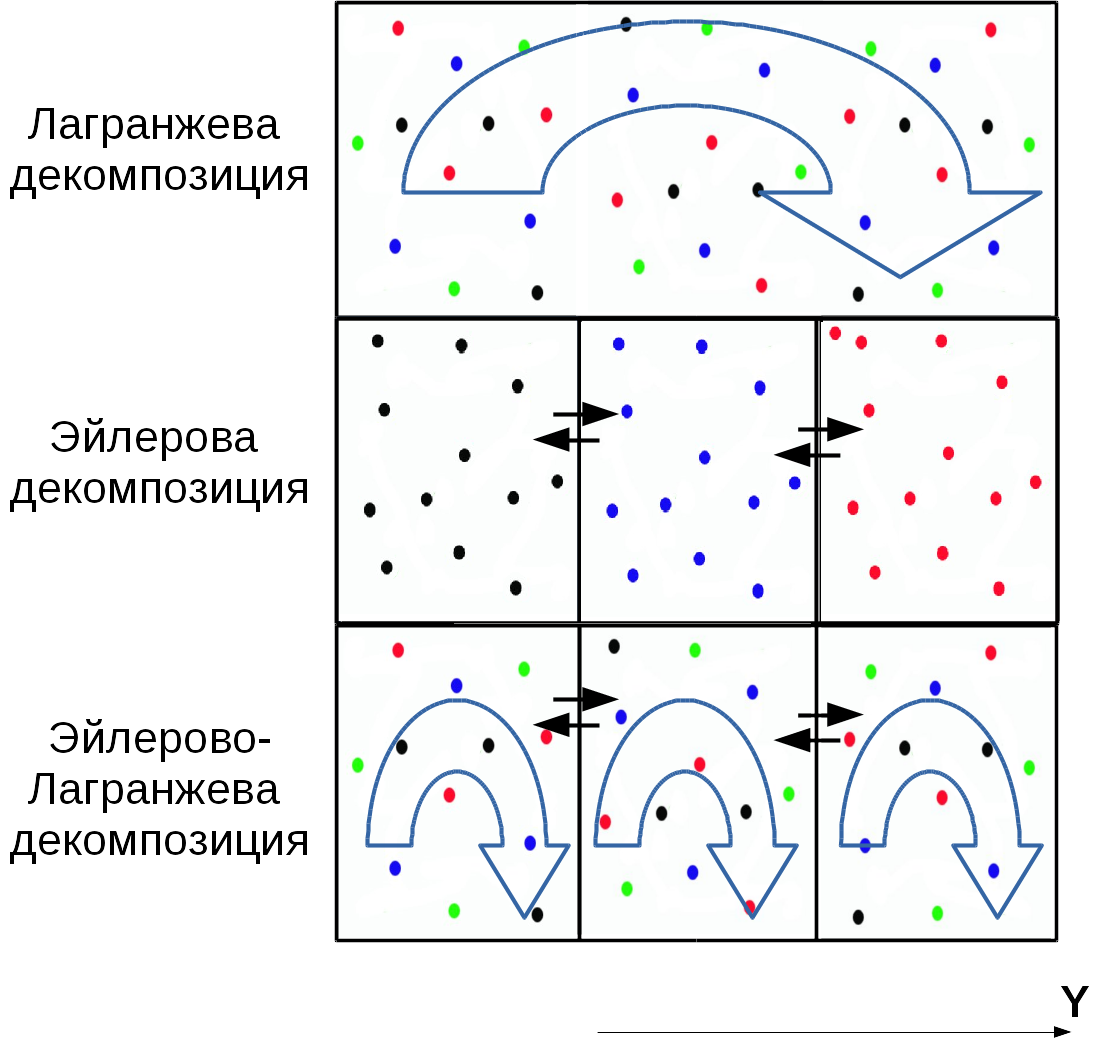
\includegraphics[height=8cm,keepaspectratio]{images/decomp_all.png}
\end{center}
\end{figure}

\clearpage

